% IPTV-Kurzanleitung, deutsche Ausgabe. In diesem Ordner erstellen mit:
%   pdflatex IPTV-Quick-Start-de.tex   (zweimal, für das Inhaltsverzeichnis)
\newcommand{\GuideLang}{ngerman}
\newcommand{\GuideTitle}{Kurzanleitung}
\newcommand{\TipLabel}{Tipp:}
% Shared layout of the IPTV quick start guides (one file per language:
% IPTV-Quick-Start.tex, IPTV-Quick-Start-it.tex, ...). Each sets, before
% % Shared layout of the IPTV quick start guides (one file per language:
% IPTV-Quick-Start.tex, IPTV-Quick-Start-it.tex, ...). Each sets, before
% % Shared layout of the IPTV quick start guides (one file per language:
% IPTV-Quick-Start.tex, IPTV-Quick-Start-it.tex, ...). Each sets, before
% \input{preamble}:
%   \GuideLang   babel language (english, italian, spanish, french, ngerman, portuguese)
%   \GuideTitle  the guide's title, used on the cover, in headers and the PDF
%   \TipLabel    the word that starts a tip box ("Tip.")
% Build any of them with pdflatex, twice (for the table of contents).
\documentclass[11pt,a4paper]{article}

\usepackage[T1]{fontenc}
\usepackage[utf8]{inputenc}
% shorthands=off: no language-specific active characters (they would clash
% with tables and addresses); only hyphenation and "Contents" etc. change.
\usepackage[shorthands=off,\GuideLang]{babel}
\usepackage{lmodern}
\usepackage[scaled=0.92]{helvet}
\renewcommand{\familydefault}{\sfdefault}
\usepackage[margin=2.2cm,headheight=14pt]{geometry}
\usepackage{graphicx}
\usepackage[table]{xcolor}
\usepackage{booktabs}
\usepackage{tabularx}
\usepackage{xltabular}
\usepackage{enumitem}
\usepackage{titlesec}
\usepackage{fancyhdr}
\usepackage{pifont}
\usepackage{amssymb}
\usepackage[hidelinks]{hyperref}

\newcommand{\version}{0.12}
\definecolor{accent}{HTML}{1E6FD9}
\definecolor{dim}{HTML}{5F6673}
\definecolor{notebg}{HTML}{EEF4FC}
\definecolor{warnbg}{HTML}{FFF6E0}
\definecolor{tvred}{HTML}{D32F2F}
\definecolor{tvgreen}{HTML}{2E7D32}
\definecolor{tvyellow}{HTML}{C9A400}
\definecolor{tvblue}{HTML}{1565C0}

\hypersetup{pdftitle={IPTV -- \GuideTitle}, pdfauthor={IPTV project}}
\setlist{itemsep=2pt, topsep=4pt}
\setlength{\parindent}{0pt}
\setlength{\parskip}{6pt}
\renewcommand{\arraystretch}{1.25}

\titleformat{\section}{\Large\bfseries\color{accent}}{\thesection}{0.6em}{}
\titleformat{\subsection}{\large\bfseries}{\thesubsection}{0.6em}{}
\titlespacing*{\section}{0pt}{14pt}{6pt}
\titlespacing*{\subsection}{0pt}{10pt}{4pt}

\pagestyle{fancy}
\fancyhf{}
\fancyhead[L]{\small\color{dim}IPTV -- \GuideTitle}
\fancyhead[R]{\small\color{dim}github.com/vickdini/iptv}
\fancyfoot[C]{\small\color{dim}\thepage}
\renewcommand{\headrulewidth}{0.4pt}
\renewcommand{\sectionmark}[1]{\markboth{#1}{}}

% A key or button on a keyboard / remote.
\newcommand{\key}[1]{{\setlength{\fboxsep}{1.5pt}\fbox{\footnotesize\vphantom{Ay}#1}}}
% A coloured remote button.
\newcommand{\colorkey}[2]{\textcolor{#1}{\ding{108}}\,\textbf{#2}}
% Shaded boxes for tips and notes.
\newcommand{\tip}[1]{\par\noindent\colorbox{notebg}{\parbox{\dimexpr\linewidth-2\fboxsep}{\small\textbf{\TipLabel} #1}}\par}
\newcommand{\note}[1]{\par\noindent\colorbox{warnbg}{\parbox{\dimexpr\linewidth-2\fboxsep}{\small #1}}\par}
\newcommand{\menu}[1]{\textit{#1}}
\newcommand{\download}{\url{https://github.com/vickdini/iptv/releases/latest}}
% Key tables: \rowcolors{2}{gray!8}{white} then
% \begin{xltabular}{\linewidth}{@{}KX@{}} \keyshead{Key}{What it does} ... \bottomrule
\newcolumntype{K}{>{\raggedright\arraybackslash}p{5.4cm}}
\newcommand{\keyshead}[2]{\toprule \textbf{#1} & \textbf{#2} \\ \midrule}

% The cover: #1 subtitle, #2 "Version".
\newcommand{\cover}[2]{%
\begin{titlepage}
  \centering
  \vspace*{0.5cm}
  {\fontsize{40}{48}\selectfont\bfseries\color{accent} IPTV\par}
  \vspace{0.3cm}
  {\LARGE \GuideTitle\par}
  \vspace{0.3cm}
  {\large\color{dim} #1\par}
  \vspace{1cm}
  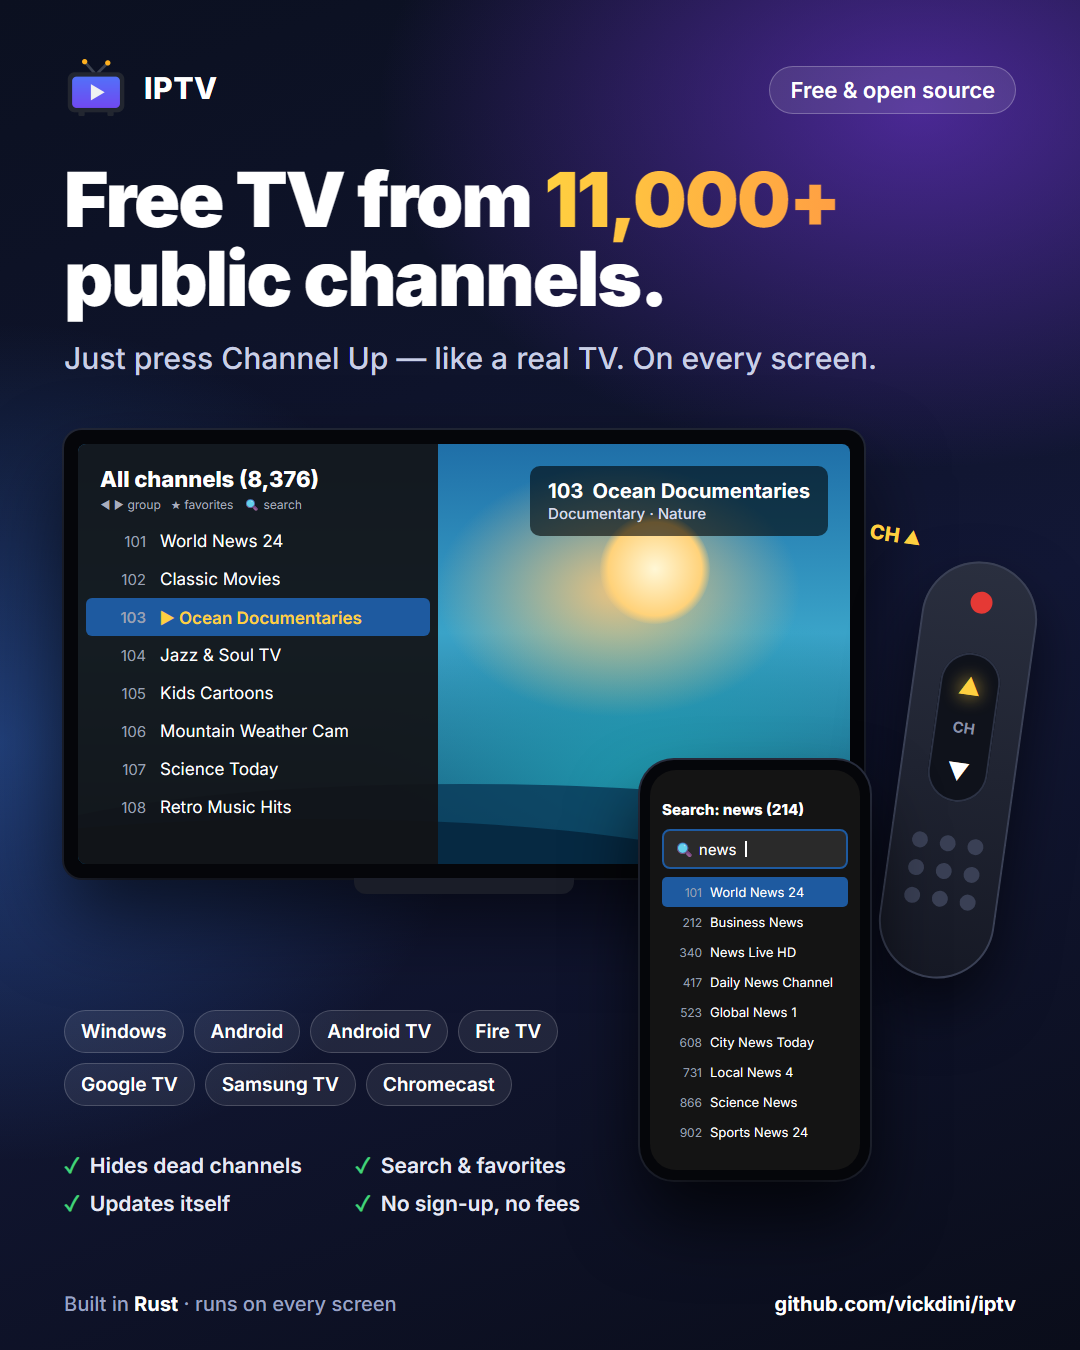
\includegraphics[width=0.52\textwidth]{../images/iptv-overview.png}\par
  \vfill
  {\large Windows \textbullet{} macOS \textbullet{} Linux \textbullet{} Android
   \textbullet{} Android TV \& Fire TV \textbullet{} Chromecast \textbullet{} Samsung TV\par}
  \vspace{0.5cm}
  {\color{dim} #2 \version{} \textbullet{} \url{https://github.com/vickdini/iptv}\par}
\end{titlepage}
\tableofcontents
\thispagestyle{fancy}}
:
%   \GuideLang   babel language (english, italian, spanish, french, ngerman, portuguese)
%   \GuideTitle  the guide's title, used on the cover, in headers and the PDF
%   \TipLabel    the word that starts a tip box ("Tip.")
% Build any of them with pdflatex, twice (for the table of contents).
\documentclass[11pt,a4paper]{article}

\usepackage[T1]{fontenc}
\usepackage[utf8]{inputenc}
% shorthands=off: no language-specific active characters (they would clash
% with tables and addresses); only hyphenation and "Contents" etc. change.
\usepackage[shorthands=off,\GuideLang]{babel}
\usepackage{lmodern}
\usepackage[scaled=0.92]{helvet}
\renewcommand{\familydefault}{\sfdefault}
\usepackage[margin=2.2cm,headheight=14pt]{geometry}
\usepackage{graphicx}
\usepackage[table]{xcolor}
\usepackage{booktabs}
\usepackage{tabularx}
\usepackage{xltabular}
\usepackage{enumitem}
\usepackage{titlesec}
\usepackage{fancyhdr}
\usepackage{pifont}
\usepackage{amssymb}
\usepackage[hidelinks]{hyperref}

\newcommand{\version}{0.12}
\definecolor{accent}{HTML}{1E6FD9}
\definecolor{dim}{HTML}{5F6673}
\definecolor{notebg}{HTML}{EEF4FC}
\definecolor{warnbg}{HTML}{FFF6E0}
\definecolor{tvred}{HTML}{D32F2F}
\definecolor{tvgreen}{HTML}{2E7D32}
\definecolor{tvyellow}{HTML}{C9A400}
\definecolor{tvblue}{HTML}{1565C0}

\hypersetup{pdftitle={IPTV -- \GuideTitle}, pdfauthor={IPTV project}}
\setlist{itemsep=2pt, topsep=4pt}
\setlength{\parindent}{0pt}
\setlength{\parskip}{6pt}
\renewcommand{\arraystretch}{1.25}

\titleformat{\section}{\Large\bfseries\color{accent}}{\thesection}{0.6em}{}
\titleformat{\subsection}{\large\bfseries}{\thesubsection}{0.6em}{}
\titlespacing*{\section}{0pt}{14pt}{6pt}
\titlespacing*{\subsection}{0pt}{10pt}{4pt}

\pagestyle{fancy}
\fancyhf{}
\fancyhead[L]{\small\color{dim}IPTV -- \GuideTitle}
\fancyhead[R]{\small\color{dim}github.com/vickdini/iptv}
\fancyfoot[C]{\small\color{dim}\thepage}
\renewcommand{\headrulewidth}{0.4pt}
\renewcommand{\sectionmark}[1]{\markboth{#1}{}}

% A key or button on a keyboard / remote.
\newcommand{\key}[1]{{\setlength{\fboxsep}{1.5pt}\fbox{\footnotesize\vphantom{Ay}#1}}}
% A coloured remote button.
\newcommand{\colorkey}[2]{\textcolor{#1}{\ding{108}}\,\textbf{#2}}
% Shaded boxes for tips and notes.
\newcommand{\tip}[1]{\par\noindent\colorbox{notebg}{\parbox{\dimexpr\linewidth-2\fboxsep}{\small\textbf{\TipLabel} #1}}\par}
\newcommand{\note}[1]{\par\noindent\colorbox{warnbg}{\parbox{\dimexpr\linewidth-2\fboxsep}{\small #1}}\par}
\newcommand{\menu}[1]{\textit{#1}}
\newcommand{\download}{\url{https://github.com/vickdini/iptv/releases/latest}}
% Key tables: \rowcolors{2}{gray!8}{white} then
% \begin{xltabular}{\linewidth}{@{}KX@{}} \keyshead{Key}{What it does} ... \bottomrule
\newcolumntype{K}{>{\raggedright\arraybackslash}p{5.4cm}}
\newcommand{\keyshead}[2]{\toprule \textbf{#1} & \textbf{#2} \\ \midrule}

% The cover: #1 subtitle, #2 "Version".
\newcommand{\cover}[2]{%
\begin{titlepage}
  \centering
  \vspace*{0.5cm}
  {\fontsize{40}{48}\selectfont\bfseries\color{accent} IPTV\par}
  \vspace{0.3cm}
  {\LARGE \GuideTitle\par}
  \vspace{0.3cm}
  {\large\color{dim} #1\par}
  \vspace{1cm}
  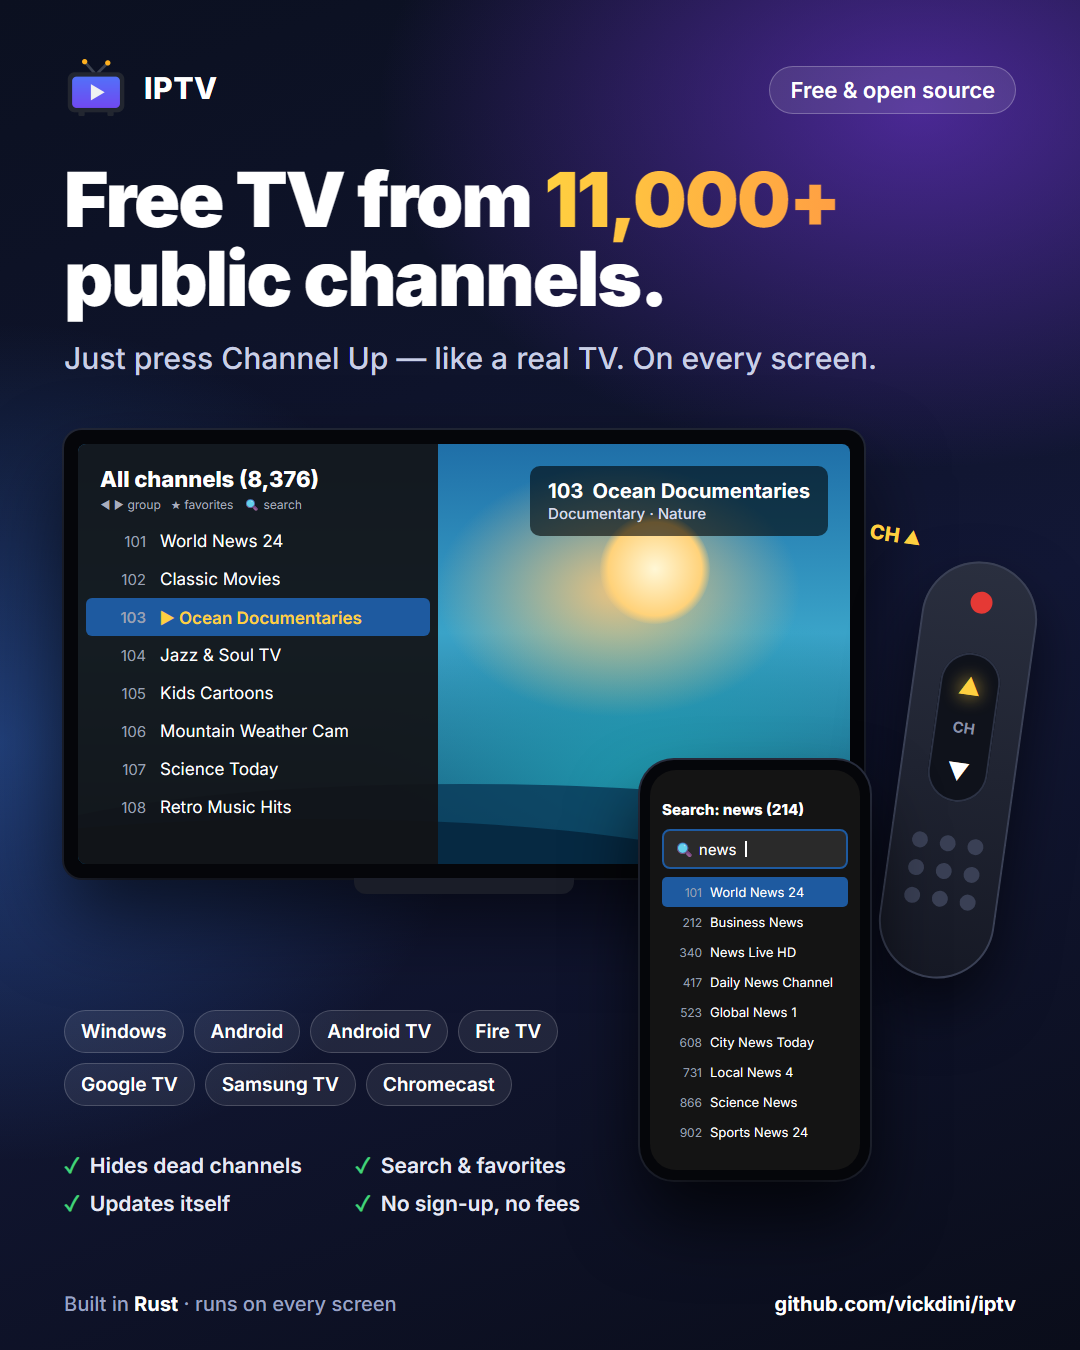
\includegraphics[width=0.52\textwidth]{../images/iptv-overview.png}\par
  \vfill
  {\large Windows \textbullet{} macOS \textbullet{} Linux \textbullet{} Android
   \textbullet{} Android TV \& Fire TV \textbullet{} Chromecast \textbullet{} Samsung TV\par}
  \vspace{0.5cm}
  {\color{dim} #2 \version{} \textbullet{} \url{https://github.com/vickdini/iptv}\par}
\end{titlepage}
\tableofcontents
\thispagestyle{fancy}}
:
%   \GuideLang   babel language (english, italian, spanish, french, ngerman, portuguese)
%   \GuideTitle  the guide's title, used on the cover, in headers and the PDF
%   \TipLabel    the word that starts a tip box ("Tip.")
% Build any of them with pdflatex, twice (for the table of contents).
\documentclass[11pt,a4paper]{article}

\usepackage[T1]{fontenc}
\usepackage[utf8]{inputenc}
% shorthands=off: no language-specific active characters (they would clash
% with tables and addresses); only hyphenation and "Contents" etc. change.
\usepackage[shorthands=off,\GuideLang]{babel}
\usepackage{lmodern}
\usepackage[scaled=0.92]{helvet}
\renewcommand{\familydefault}{\sfdefault}
\usepackage[margin=2.2cm,headheight=14pt]{geometry}
\usepackage{graphicx}
\usepackage[table]{xcolor}
\usepackage{booktabs}
\usepackage{tabularx}
\usepackage{xltabular}
\usepackage{enumitem}
\usepackage{titlesec}
\usepackage{fancyhdr}
\usepackage{pifont}
\usepackage{amssymb}
\usepackage[hidelinks]{hyperref}

\newcommand{\version}{0.12}
\definecolor{accent}{HTML}{1E6FD9}
\definecolor{dim}{HTML}{5F6673}
\definecolor{notebg}{HTML}{EEF4FC}
\definecolor{warnbg}{HTML}{FFF6E0}
\definecolor{tvred}{HTML}{D32F2F}
\definecolor{tvgreen}{HTML}{2E7D32}
\definecolor{tvyellow}{HTML}{C9A400}
\definecolor{tvblue}{HTML}{1565C0}

\hypersetup{pdftitle={IPTV -- \GuideTitle}, pdfauthor={IPTV project}}
\setlist{itemsep=2pt, topsep=4pt}
\setlength{\parindent}{0pt}
\setlength{\parskip}{6pt}
\renewcommand{\arraystretch}{1.25}

\titleformat{\section}{\Large\bfseries\color{accent}}{\thesection}{0.6em}{}
\titleformat{\subsection}{\large\bfseries}{\thesubsection}{0.6em}{}
\titlespacing*{\section}{0pt}{14pt}{6pt}
\titlespacing*{\subsection}{0pt}{10pt}{4pt}

\pagestyle{fancy}
\fancyhf{}
\fancyhead[L]{\small\color{dim}IPTV -- \GuideTitle}
\fancyhead[R]{\small\color{dim}github.com/vickdini/iptv}
\fancyfoot[C]{\small\color{dim}\thepage}
\renewcommand{\headrulewidth}{0.4pt}
\renewcommand{\sectionmark}[1]{\markboth{#1}{}}

% A key or button on a keyboard / remote.
\newcommand{\key}[1]{{\setlength{\fboxsep}{1.5pt}\fbox{\footnotesize\vphantom{Ay}#1}}}
% A coloured remote button.
\newcommand{\colorkey}[2]{\textcolor{#1}{\ding{108}}\,\textbf{#2}}
% Shaded boxes for tips and notes.
\newcommand{\tip}[1]{\par\noindent\colorbox{notebg}{\parbox{\dimexpr\linewidth-2\fboxsep}{\small\textbf{\TipLabel} #1}}\par}
\newcommand{\note}[1]{\par\noindent\colorbox{warnbg}{\parbox{\dimexpr\linewidth-2\fboxsep}{\small #1}}\par}
\newcommand{\menu}[1]{\textit{#1}}
\newcommand{\download}{\url{https://github.com/vickdini/iptv/releases/latest}}
% Key tables: \rowcolors{2}{gray!8}{white} then
% \begin{xltabular}{\linewidth}{@{}KX@{}} \keyshead{Key}{What it does} ... \bottomrule
\newcolumntype{K}{>{\raggedright\arraybackslash}p{5.4cm}}
\newcommand{\keyshead}[2]{\toprule \textbf{#1} & \textbf{#2} \\ \midrule}

% The cover: #1 subtitle, #2 "Version".
\newcommand{\cover}[2]{%
\begin{titlepage}
  \centering
  \vspace*{0.5cm}
  {\fontsize{40}{48}\selectfont\bfseries\color{accent} IPTV\par}
  \vspace{0.3cm}
  {\LARGE \GuideTitle\par}
  \vspace{0.3cm}
  {\large\color{dim} #1\par}
  \vspace{1cm}
  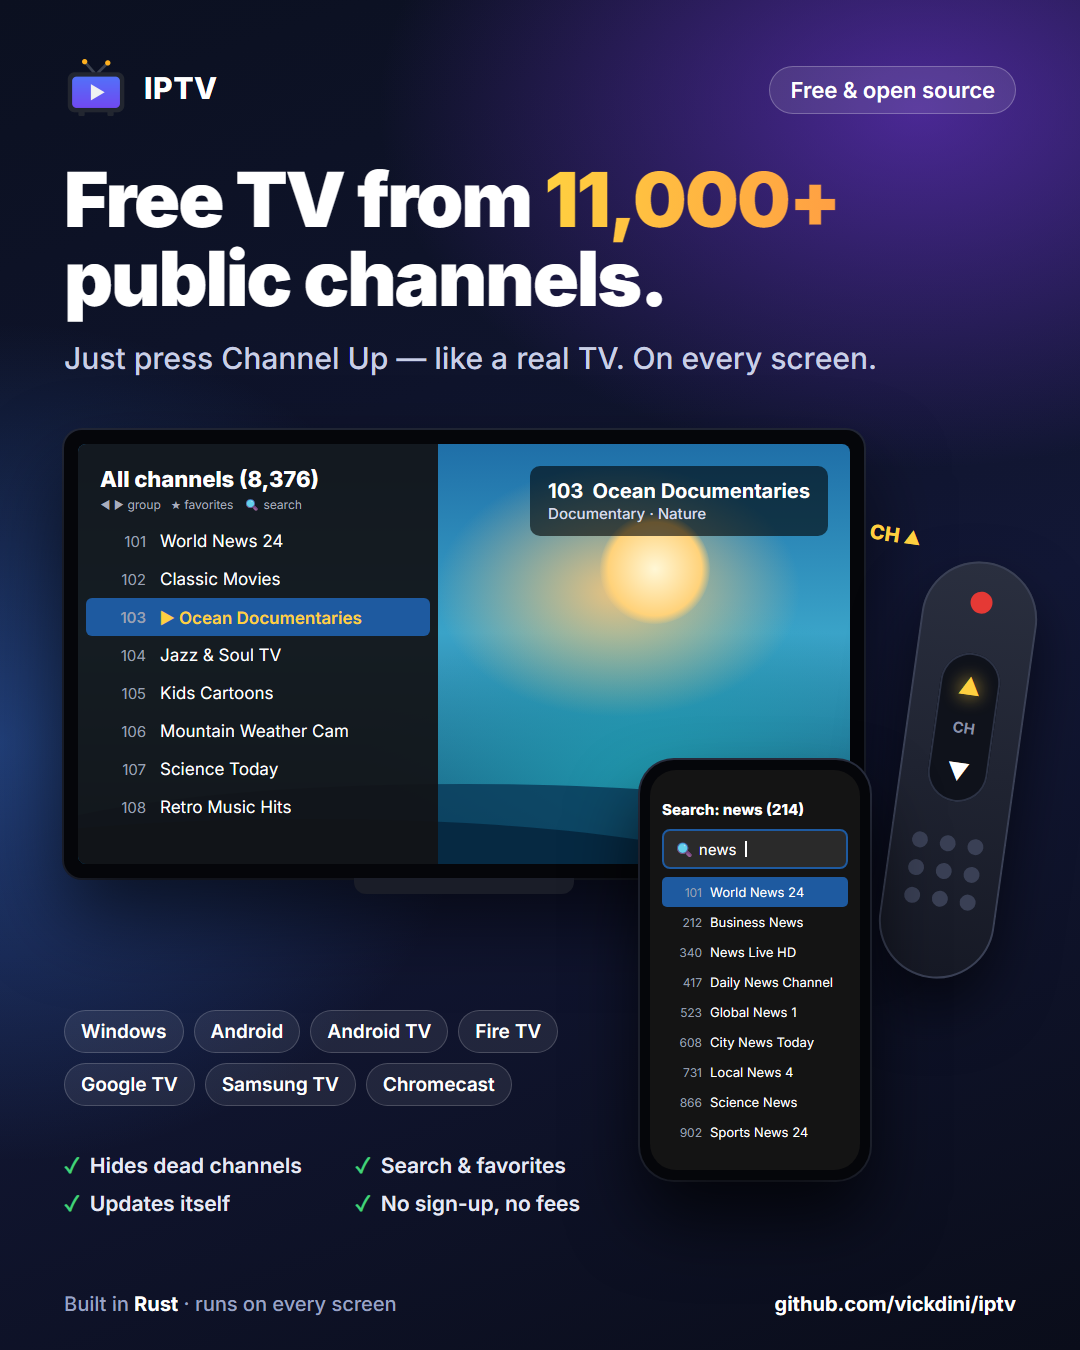
\includegraphics[width=0.52\textwidth]{../images/iptv-overview.png}\par
  \vfill
  {\large Windows \textbullet{} macOS \textbullet{} Linux \textbullet{} Android
   \textbullet{} Android TV \& Fire TV \textbullet{} Chromecast \textbullet{} Samsung TV\par}
  \vspace{0.5cm}
  {\color{dim} #2 \version{} \textbullet{} \url{https://github.com/vickdini/iptv}\par}
\end{titlepage}
\tableofcontents
\thispagestyle{fancy}}


\begin{document}
\cover{Kostenlose Fernsehsender ansehen und zappen wie am Fernseher}{Version}

% ------------------------------------------------------------------ intro
\section{Über IPTV}

IPTV spielt die kostenlosen, öffentlich gelisteten Fernsehsender ab, die das
Projekt \emph{iptv-org} sammelt (mehr als 10\,000), und lässt dich zwischen
ihnen wechseln wie am Fernseher: Sender vor und zurück, Sendernummern,
Favoriten und Gruppen wie Nachrichten, Filme oder Sport.

\begin{itemize}
  \item \textbf{Immer aktuell.} Die Senderliste wird bei jedem Start
        aktualisiert, und die App aktualisiert sich selbst, wenn eine neue
        Version erscheint.
  \item \textbf{Nur Sender, die funktionieren.} Sender, die gerade nicht
        senden, werden automatisch ausgeblendet -- so bleibt das Zappen nie
        auf einem schwarzen Bild hängen.
  \item \textbf{Sender schnell finden.} Suche nach Namen, erkenne jeden
        Sender an seinem Logo, kehre zu zuletzt gesehenen Sendern zurück
        oder zeige nur die Länder und Sprachen, die dich interessieren.
  \item \textbf{Deine Sprache.} IPTV spricht Deutsch, Englisch,
        Italienisch, Spanisch, Französisch und Portugiesisch und folgt der
        Sprache deines Geräts. Bei Sendern, die das anbieten, wählst du die
        Audiosprache und schaltest Untertitel ein.
  \item \textbf{Handy-Fernbedienung.} Steuere den Fernseher oder Computer
        über den Browser deines Handys (Abschnitt~\ref{sec:remote}).
\end{itemize}

Jeder Download enthält alles Nötige: Es muss nichts weiter installiert
werden. Alle Downloads findest du auf der Release-Seite:

\begin{center}
  \download
\end{center}

\note{\textbf{Hinweis.} IPTV stellt selbst keine Videos bereit: Es lädt nur
eine öffentlich verfügbare Senderliste des Projekts iptv-org. Sieh dir nur
an, was du in deinem Land legal ansehen darfst.}

% ------------------------------------------------------------------ Windows
\section{Windows}
\label{sec:windows}

\subsection{Installation}
\begin{enumerate}
  \item Lade \texttt{IPTV-Setup-\textless Version\textgreater.exe} von der
        Release-Seite herunter und öffne die Datei.
  \item Wenn Windows \menu{Der Computer wurde durch Windows geschützt}
        meldet, klicke auf \menu{Weitere Informationen} und dann auf
        \menu{Trotzdem ausführen}.
  \item Folge dem Installationsprogramm. Es braucht keine
        Administratorrechte und legt eine Verknüpfung im Startmenü an (und
        auf Wunsch ein Symbol auf dem Desktop).
\end{enumerate}
IPTV öffnet sich maximiert und spielt sofort ab. Zum Entfernen gehst du auf
\menu{Einstellungen \textrightarrow{} Apps}.

\subsection{Tasten}
\label{sec:keys}
Diese Tasten funktionieren auf jedem Computer: Windows, macOS und Linux.

\rowcolors{2}{gray!8}{white}
\begin{xltabular}{\linewidth}{@{}KX@{}}
\keyshead{Taste}{Funktion}
\key{$\uparrow$} \key{$\downarrow$}, \key{Bild$\uparrow$} \key{Bild$\downarrow$}, Mausrad & nächster / vorheriger Sender \\
\key{0}--\key{9}, dann warten oder \key{Enter} & zu einer Sendernummer \\
\key{Rücktaste} & zurück zum vorherigen Sender \\
\key{$\leftarrow$} \key{$\rightarrow$}, \key{m} & leiser / lauter, stumm \\
\key{l}, \key{Tab} oder Rechtsklick & Senderliste öffnen / schließen \\
\key{/} oder \key{Strg}+\key{F} & Sender nach Namen suchen \\
\key{c} & Länder und Sprachen wählen \\
\key{g} / \key{G} & zuletzt gesehen, dann die Gruppen (Nachrichten, Filme\ldots) \\
\key{s} / \key{S} & Favorit hinzufügen oder entfernen / nur durch Favoriten zappen \\
\key{a} / \key{t} & nächste Audiosprache / nächste Untertitel (und aus) \\
\key{r} & Handy-Fernbedienung: QR-Code anzeigen \\
\key{E} / \key{I} & Favoriten exportieren / importieren (Ordner Downloads) \\
\key{i} & Senderinfo \\
\key{f}, Doppelklick & Vollbild (\key{Esc} beendet es) \\
\key{p} & Bild im Bild: ein zweiter Sender, klein, unten rechts in der Ecke \\
\key{[} / \key{]} & vorheriger / nächster Sender des kleinen Bildes \\
\key{x}, Klick auf das kleine Bild & die beiden Sender tauschen \\
\key{Leertaste} & Pause \\
\key{h}, \key{?} oder \key{F1} & Hilfe auf dem Bildschirm \\
\key{q} & beenden \\
\bottomrule
\end{xltabular}

\subsection{Die Senderliste}
Drücke \key{l}, um links eine scrollbare Senderliste mit Logos zu öffnen;
das Video läuft daneben weiter. Blättere mit dem Mausrad und klicke auf einen
Sender, um ihn anzusehen. Tippe einfach los (oder drücke \key{/}), um zu
suchen: Akzente und Groß-/Kleinschreibung spielen keine Rolle. \key{Esc}
schließt die Liste. Drücke \key{g} für die zuletzt gesehenen Sender, den
neuesten zuerst.

\subsection{Länder und Sprachen}
Drücke \key{c}, tippe, um ein Land oder eine Sprache zu finden, und drücke
\key{Enter}, um es anzukreuzen; \key{Tab} wechselt zwischen den beiden
Listen. Danach zeigt IPTV nur noch Sender aus den angekreuzten Ländern oder
in den angekreuzten Sprachen, bis du die Auswahl löschst (\key{Entf} oder die
Zeile \emph{Alle Filter löschen}).

\subsection{Audiosprache und Untertitel}
Bietet ein Sender mehrere Audiosprachen oder Untertitel, weist ein Hinweis
unten im Bild darauf hin. Drücke \key{a} für die nächste Audiosprache und
\key{t} für die nächsten Untertitel (und zuletzt \emph{aus}). IPTV merkt sich
die Sprache und verwendet sie bei allen anderen Sendern, die sie anbieten.

\subsection{Sprache und Updates}
IPTV verwendet die Systemsprache. Bei jedem Start prüft es, ob es eine neue
Version gibt; wenn ja, installiert es sie ohne Rückfrage und startet nach
wenigen Sekunden von selbst neu.

% ------------------------------------------------------------------ macOS
\section{macOS}

\subsection{Installation}
\begin{enumerate}
  \item Finde heraus, welchen Chip dein Mac hat: \menu{Apple-Menü
        \textrightarrow{} Über diesen Mac}.
  \item Lade das passende Image von der Release-Seite herunter:
  \begin{itemize}
    \item Apple Silicon (M1, M2, M3, M4\ldots):
          \texttt{IPTV-\textless Version\textgreater-macOS-arm64.dmg}
    \item Intel: \texttt{IPTV-\textless Version\textgreater-macOS-x86\_64.dmg}
  \end{itemize}
  \item Öffne es und ziehe \textbf{IPTV} auf \textbf{Programme}.
\end{enumerate}

\subsection{Erster Start}
IPTV ist nicht von Apple beglaubigt, deshalb verweigert macOS beim ersten
Mal das Öffnen. Das ist nur einmal nötig:
\begin{enumerate}
  \item Öffne IPTV aus dem Ordner Programme. Wenn macOS meldet, dass es
        nicht geöffnet werden kann, klicke auf \menu{Fertig}.
  \item Öffne \menu{Systemeinstellungen \textrightarrow{} Datenschutz \&
        Sicherheit}, scrolle zu \menu{„IPTV“ wurde blockiert\ldots} und klicke
        auf \menu{Dennoch öffnen}; bestätige dann.
\end{enumerate}

\subsection{Verwendung}
IPTV verwendet dieselben Tasten wie unter Windows
(Abschnitt~\ref{sec:keys}). Im Dock erscheint es als \textbf{IPTV}, solange
ein Sender läuft.

\tip{Lass IPTV im Ordner Programme: Aus dem Image oder dem Ordner Downloads
gestartet, führt macOS es aus einer schreibgeschützten Kopie aus, und es
kann sich nicht aktualisieren.}

% ------------------------------------------------------------------ Linux
\section{Linux}

\subsection{Installation}
Lade \texttt{IPTV-\textless Version\textgreater-x86\_64.AppImage} von der
Release-Seite herunter. Das ist eine einzige Datei, die alles enthält. Mach
sie ausführbar und starte sie:
\begin{center}
\begin{minipage}{0.8\linewidth}
\small\ttfamily chmod +x IPTV-*-x86\_64.AppImage\\
./IPTV-*-x86\_64.AppImage
\end{minipage}
\end{center}
Alternativ öffnest du im Dateimanager \menu{Eigenschaften \textrightarrow{}
Zugriffsrechte}, setzt den Haken bei \menu{Datei als Programm ausführen
erlauben} und doppelklickst die Datei.

Es läuft auf 64-Bit-PCs mit einem Linux von 2022 oder neuer (Ubuntu 22.04,
Debian 12, Fedora 36, Linux Mint 21 und neuer).

\tip{Werkzeuge wie \emph{Gear Lever} oder \emph{AppImageLauncher} fügen IPTV
dem Anwendungsmenü hinzu. Meldet das AppImage, dass FUSE fehlt, starte es
mit \texttt{-{}-appimage-extract-and-run}.}

\subsection{Verwendung}
IPTV verwendet dieselben Tasten wie unter Windows
(Abschnitt~\ref{sec:keys}). Es aktualisiert sich, indem es die AppImage-Datei
ersetzt -- bewahre sie also in einem Ordner auf, in den du schreiben darfst
(zum Beispiel in deinem Benutzerordner).

% ------------------------------------------------------------------ Android
\section{Android-Handys und -Tablets}

\subsection{Installation}
\begin{enumerate}
  \item Lade auf dem Handy \texttt{IPTV-\textless Version\textgreater.apk}
        von der Release-Seite herunter und öffne die Datei.
  \item Android fragt einmal, ob Apps aus dem Browser oder Dateimanager
        installiert werden dürfen: Erlaube es und tippe auf
        \menu{Installieren}.
  \item IPTV ist nicht bei Google Play, daher warnt Play Protect eventuell
        vor einem unbekannten Entwickler: Wähle \menu{Trotzdem
        installieren}.
\end{enumerate}
Du kannst es auch mit \emph{Obtainium} installieren, das Apps direkt von
ihrer Release-Seite aktuell hält.

\subsection{Gesten}
\rowcolors{2}{gray!8}{white}
\begin{xltabular}{\linewidth}{@{}KX@{}}
\keyshead{Geste}{Funktion}
nach oben / unten wischen & nächster / vorheriger Sender \\
tippen & Senderliste öffnen / schließen \\
doppelt tippen & zurück zum vorherigen Sender \\
lange drücken & Senderinfo \\
\bottomrule
\end{xltabular}

\subsection{Zwei Sender gleichzeitig}
Halte das Handy oder Tablet hochkant, dann teilt sich der Bildschirm in zwei
Sender übereinander. Tippe auf eine Hälfte, um sie zu hören: Ein dünner blauer
Rahmen markiert sie, und die Senderliste und die Handy-Fernbedienung wirken
auf sie. Wische auf einer Hälfte nach oben oder unten, um ihren Sender zu
wechseln. Dreh das Gerät wieder quer für einen einzigen Sender.

\subsection{Bild im Bild}
Verlasse die App während der Wiedergabe (Home-Taste oder vom unteren Rand
nach oben wischen): Der Sender läuft in einem kleinen Fenster über deinen
anderen Apps weiter, mit Tasten zum Senderwechsel. Tippe auf das Fenster, um
zu IPTV zurückzukehren, oder zieh es weg, um es zu schließen. Benötigt
Android 8 oder neuer.

\subsection{Die Senderliste}
Tippe auf den Bildschirm, um sie zu öffnen. Tippe auf einen Sender, um ihn
anzusehen; lange drücken fügt ihn zu den Favoriten hinzu oder entfernt ihn.
Die Schaltflächen oben:
\begin{itemize}
  \item \textbf{Suchfeld}: Gib einen Teil des Sendernamens ein.
  \item Pfeile $\blacktriangleleft$\,$\blacktriangleright$: vorherige /
        nächste Gruppe.
  \item \textbf{Uhr}: die zuletzt gesehenen Sender.
  \item $\bigstar$: nur Favoriten. Lange drücken, um die Favoriten in einer
        Datei zu speichern oder aus einer Datei hinzuzufügen.
  \item \textbf{Globus}: Länder und Sprachen wählen.
  \item \textbf{Untertitel} (nur bei Sendern mit Auswahl): Audiosprache und
        Untertitel.
  \item \textbf{Handy-Fernbedienung}: IPTV von einem anderen Handy steuern
        (Abschnitt~\ref{sec:remote}).
  \item \textbf{Streamen}: auf einem Chromecast abspielen
        (Abschnitt~\ref{sec:chromecast}).
  \item \textbf{Beenden}: schließt IPTV (und beendet das Streamen).
\end{itemize}

\subsection{Sprache und Updates}
IPTV verwendet die Sprache deines Handys. Beim Start prüft es, ob es eine
neue Version gibt. Beim ersten Mal fragt Android, ob IPTV Apps installieren
darf; danach werden Updates mit höchstens einer Bestätigung installiert.

% ------------------------------------------------------------------ Android TV
\section{Android TV, Google TV und Fire TV}

Dieselbe App läuft auf TV-Geräten und wird mit der Fernbedienung bedient. Die
TV-Stores bieten sie nicht an, daher wird sie einmalig mit der kostenlosen
App \emph{Downloader} installiert:

\begin{itemize}
  \item \textbf{Fire TV / Fire TV Stick:} Installiere \emph{Downloader} aus
        dem Amazon-Store. Öffne dann \menu{Einstellungen \textrightarrow{}
        Mein Fire TV \textrightarrow{} Entwickleroptionen \textrightarrow{}
        Unbekannte Apps installieren} und aktiviere Downloader.
  \item \textbf{Google TV, Chromecast mit Google TV, Android TV:} Installiere
        \emph{Downloader} aus dem Play Store und erlaube es unter
        \menu{Einstellungen \textrightarrow{} Apps \textrightarrow{}
        Sicherheit \& Einschränkungen \textrightarrow{} Unbekannte Quellen}.
\end{itemize}
Gib in Downloader
\begin{center}
  \download
\end{center}
ein, lade dann \texttt{IPTV-\textless Version\textgreater.apk} herunter und
installiere sie. IPTV erscheint danach bei den Apps des Fernsehers.

\subsection{Fernbedienung}
\rowcolors{2}{gray!8}{white}
\begin{xltabular}{\linewidth}{@{}KX@{}}
\keyshead{Taste}{Funktion}
Hoch / Runter, Kanal +/$-$, Vor- / Zurückspulen & nächster / vorheriger Sender \\
OK, Wiedergabe/Pause, Menü & Senderliste öffnen / schließen \\
Links / Rechts & zuletzt gesehen, dann die Gruppen \\
0--9 (falls vorhanden) & zu einer Sendernummer \\
Zurück & Liste schließen \\
Info & Senderinfo \\
Audio- / CC-Tasten (falls vorhanden) & nächste Audiosprache / Untertitel \\
\bottomrule
\end{xltabular}

Drücke in der Senderliste beim ersten Sender auf Hoch, um ins Suchfeld zu
gelangen. Die Schaltflächen oben in der Liste wählen Länder und Sprachen,
Audio und Untertitel und öffnen die Handy-Fernbedienung.

\tip{Die meisten dieser Fernbedienungen haben keine Zifferntasten: Mit der
Handy-Fernbedienung (Abschnitt~\ref{sec:remote}) wählst du am schnellsten
einen Sender.}

% ------------------------------------------------------------------ Chromecast
\section{Chromecast}
\label{sec:chromecast}

Ältere Chromecasts (der einfache Stick ohne Fernbedienung) können keine Apps
installieren. Streame stattdessen aus der Android-App auf sie:
\begin{enumerate}
  \item Achte darauf, dass Handy und Chromecast im selben WLAN sind.
  \item Öffne in IPTV die Senderliste, tippe auf die Schaltfläche
        \textbf{Streamen} und wähle deinen Chromecast.
  \item Zappe wie gewohnt auf dem Handy: Der Fernseher folgt.
\end{enumerate}
Manche Sender lassen sich nicht streamen, weil ihre Server das nicht
erlauben; IPTV überspringt sie automatisch.

% ------------------------------------------------------------------ Samsung
\section{Samsung-Smart-TVs}

IPTV läuft auf Samsung-Fernsehern ab Baujahr 2019. Samsung erlaubt Apps, die
nicht im eigenen Store sind, nur über einen Computer zu installieren, mit
dem Fernseher im \emph{Entwicklermodus}. Die Einrichtung erfolgt einmalig
von einem Windows-PC im selben WLAN wie der Fernseher.

\subsection{Installation}
\begin{enumerate}
  \item Installiere auf dem PC die Kommandozeilenwerkzeuge von \emph{Tizen
        Studio} von \url{https://developer.tizen.org}. Installiere in dessen
        Package Manager \emph{Samsung Certificate Extension} und \emph{TV
        Extensions Tools} (Registerkarte \menu{Extension SDK}).
  \item Öffne auf dem Fernseher \menu{Apps} und gib mit der Fernbedienung
        \key{1}\key{2}\key{3}\key{4}\key{5} ein. Schalte den
        \menu{Entwicklermodus} ein, gib die IP-Adresse des PCs ein und
        starte den Fernseher neu.
  \item Lade \texttt{IPTV-Samsung-TV-\textless Version\textgreater.zip} von
        der Release-Seite herunter und entpacke sie.
  \item Ermittle die IP-Adresse des Fernsehers (\menu{Einstellungen
        \textrightarrow{} Allgemein \textrightarrow{} Netzwerk
        \textrightarrow{} Netzwerkstatus}) und führe im entpackten Ordner aus:
\begin{center}
\begin{minipage}{0.92\linewidth}
\small\ttfamily powershell -ExecutionPolicy Bypass -File install-on-tv.ps1 -TvIp 192.168.1.4
\end{minipage}
\end{center}
        Beim ersten Mal erklärt es, wie du das kostenlose Samsung-Zertifikat
        erstellst (mit einem Samsung-Konto). Führe es danach noch einmal aus:
        Es installiert IPTV, das dann bei den Apps des Fernsehers erscheint.
\end{enumerate}
Danach aktualisiert sich IPTV selbst: Für neue Versionen musst du die
Einrichtung nicht wiederholen. Es verwendet die Sprache des Fernsehers.

\subsection{Fernbedienung}
\rowcolors{2}{gray!8}{white}
\begin{xltabular}{\linewidth}{@{}KX@{}}
\keyshead{Taste}{Funktion}
Hoch / Runter, CH + / CH $-$ & nächster / vorheriger Sender \\
0--9 & zu einer Sendernummer \\
OK & Senderliste (in der Liste: ausgewählten Sender ansehen) \\
Links / Rechts & zuletzt gesehen, dann die Gruppen \\
PRE-CH & zurück zum vorherigen Sender \\
INFO & Senderinfo \\
\colorkey{tvred}{Rot} & Favorit hinzufügen oder entfernen \\
\colorkey{tvgreen}{Grün} & nur Favoriten \\
\colorkey{tvyellow}{Gelb} & Menü für Audiosprache und Untertitel \\
\colorkey{tvyellow}{Gelb} in der Liste & Länder und Sprachen wählen \\
\colorkey{tvblue}{Blau} & Sender nach Namen suchen \\
Zurück & Liste schließen oder IPTV verlassen \\
\bottomrule
\end{xltabular}

\note{Die Handy-Fernbedienung (Abschnitt~\ref{sec:remote}) gibt es auf
Samsung-Fernsehern noch nicht. Die kostenlose App \emph{SmartThings}
funktioniert für die Grundtasten als Fernbedienung auf dem Handy.}

% ------------------------------------------------------------------ remote
\section{Handy-Fernbedienung}
\label{sec:remote}

Steuere IPTV mit deinem Handy, Android oder iPhone, ohne etwas zu
installieren. Du kannst alle Sender durchblättern und durchsuchen und einen
antippen, um ihn anzusehen; dazu kommen Favoriten, zuletzt gesehene Sender,
Sender vor / zurück, Lautstärke, Audiosprache und Untertitel. Sie
funktioniert mit IPTV auf einem Computer und auf Android TV, Google TV und
Fire TV und spricht die Sprache deines Handys.

\begin{enumerate}
  \item Drücke am Computer \key{r}. Öffne auf Android TV, Google TV oder
        Fire TV die Senderliste und wähle die Schaltfläche
        \textbf{Handy-Fernbedienung}. Ein QR-Code erscheint.
  \item Scanne ihn mit der Handykamera. Das Handy muss im selben WLAN sein.
        Ohne Kamera öffnest du im Browser des Handys die angezeigte Adresse
        und gibst die PIN ein.
  \item Die Fernbedienung öffnet sich im Browser des Handys. Füge sie zum
        Startbildschirm oder zu den Lesezeichen hinzu: Ab dann verbindet sie
        sich von selbst, sobald IPTV läuft.
\end{enumerate}

Um deine Favoriten auf einen anderen Fernseher oder Computer zu übertragen,
verwende \textbf{Auf dem Handy speichern} unten auf der Seite der
Fernbedienung und dann \textbf{Aus Datei hinzufügen} in der Fernbedienung
des anderen Geräts. Favoriten werden hinzugefügt, nie entfernt. Am Computer
kannst du auch \key{E} drücken (im Ordner Downloads speichern) und \key{I}
(von dort hinzufügen); auf Android-Handys und -Tablets drückst du lange auf
die Schaltfläche $\bigstar$.

\note{Beim ersten Mal fragt Windows (und macOS, wenn die Firewall aktiv ist),
ob IPTV das Netzwerk nutzen darf: Erlaube es in \textbf{privaten} Netzwerken,
sonst können sich Handys nicht verbinden. Nur Handys, die die PIN kennen,
können IPTV steuern.}

% ------------------------------------------------------------------ help
\section{Fehlerbehebung}

\begin{description}[style=nextline, leftmargin=0pt, itemsep=6pt]
  \item[Ein Sender spielt nicht.] Viele kostenlose Sender gehen offline oder
        funktionieren nur in manchen Ländern. IPTV blendet sie aus und
        wechselt von selbst weiter; wechsle einfach den Sender.
  \item[Die Liste ist kürzer als vorher.] Prüfe, ob Länder oder Sprachen
        ausgewählt sind (\key{c} am Computer, der Globus unter Android,
        \colorkey{tvyellow}{Gelb} in der Liste auf Samsung-Fernsehern), und
        lösche die Auswahl.
  \item[Die Handy-Fernbedienung verbindet sich nicht.] Achte darauf, dass das
        Handy im selben WLAN ist (nicht im Mobilfunknetz) und dass die
        Firewall des Computers IPTV in privaten Netzwerken erlaubt.
  \item[Untertitel werden angezeigt, aber es erscheint nichts.] Manche Sender
        kündigen Untertitel an, die sie gar nicht senden. An IPTV liegt es
        nicht.
  \item[IPTV ist in der falschen Sprache.] Es folgt der Sprache des Geräts
        (am Computer der Systemsprache). Namen von Sendern, Gruppen und
        Ländern stammen aus der Senderliste und sind immer auf Englisch.
  \item[Etwas anderes?] Melde es unter
        \url{https://github.com/vickdini/iptv/issues}.
\end{description}

\vfill
{\small\color{dim} IPTV ist freie Software unter der GNU General Public
License, Version 3 oder neuer. Der Quellcode liegt unter
\url{https://github.com/vickdini/iptv}.\par}

\end{document}
